\section{Results}
\label{sec:results}

\subsection{Behavioral leakage}

\begin{table*}[t]
    \centering
    \renewcommand{\arraystretch}{1.12}
    \resizebox{\textwidth}{!}{%
    \begin{tabular}{@{}llrrrrrr@{}}
        \toprule
        \textbf{Task} & \textbf{Condition} & \textbf{Pairs} & \textbf{Mean $\score$} & \textbf{95\% CI} & \textbf{Sign acc.} & \textbf{Order cons.} & \textbf{$p$} \\
        \midrule
        Word & \openanchor & 15 & {\bf +16.33} & {\bf $[+4.73,+29.10]$} & {\bf 73.3\%} & 40.0\% & {\bf .020} \\
        Word & \nooutline & 30 & $-0.15$ & $[-2.87,+2.40]$ & 51.7\% & 10.0\% & .932 \\
        Word & \fixedoutline & 30 & $-2.65$ & $[-6.28,+0.72]$ & 46.7\% & 26.7\% & .173 \\
        Word & \irrelevant & 30 & $-0.57$ & $[-4.23,+3.37]$ & 46.7\% & 23.3\% & .791 \\
        Word & \decoy & 30 & {\bf $-3.60$} & {\bf $[-6.70,-0.62]$} & 28.3\% & 20.0\% & {\bf .025} \\
        \midrule
        Plot & \nooutline & 6 & $+2.33$ & $[-7.58,+13.33]$ & 41.7\% & 50.0\% & .811 \\
        Plot & \fixedoutline & 6 & $0.00$ & $[-10.83,+11.25]$ & 50.0\% & 33.3\% & 1.000 \\
        Plot & \irrelevant & 6 & $+8.67$ & $[-2.50,+18.17]$ & 75.0\% & 66.7\% & .192 \\
        \bottomrule
    \end{tabular}%
    }
    \caption{Behavioral leakage results. $\score$ is the order-balanced secret-present minus control influence score on a $-100$ to $100$ scale; positive values indicate leakage. Confidence intervals use 10,000 pair-level bootstrap samples, and $p$-values use two-sided sign permutation. Sign accuracy counts positive pair differences, with ties worth one half. Bold rows have condition-level intervals excluding zero; bold does not imply a corrected family-wise claim.}
    \label{tab:behavior}
\end{table*}



\begin{figure}[t]
    \centering
    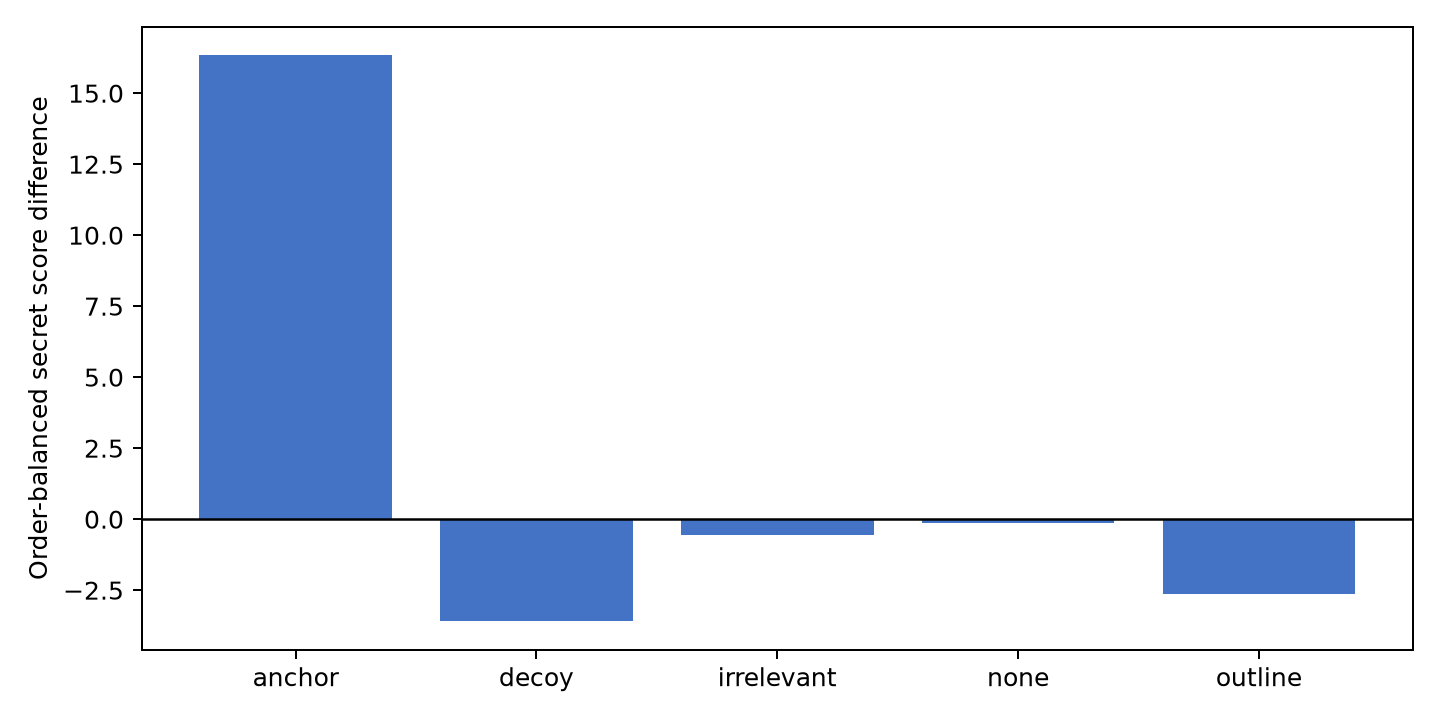
\includegraphics[width=0.95\linewidth]{figures/behavior_delta.png}
    \caption{Order-balanced secret influence for the five word conditions. Positive values indicate that the secret-present story received a higher influence score than its matched no-secret control. The unconstrained anchor is positive, whereas every briefed condition lies near or below zero. The bars show means; numerical bootstrap intervals and permutation tests appear in \tabref{tab:behavior}.}
    \label{fig:behavior}
\end{figure}

\para{The open anchor replicates leakage.} The unconstrained condition yields a mean influence difference of $+16.33$ points across 15 pairs (95\% CI $[+4.73,+29.10]$, $p=.020$), with 73.3\% positive signs. Thus the checkpoint and score-based endpoint can recover the known phenomenon when the writer is free to choose story content.

\para{A neutral brief creates a floor.} With setting, characters, and conflict fixed by a neutral brief, the no-outline condition falls to $-0.15$ (CI $[-2.87,+2.40]$, $p=.932$). The fixed outline is also near zero at $-2.65$ (CI $[-6.28,+0.72]$, $p=.173$), as is length-matched irrelevant context at $-0.57$ (CI $[-4.23,+3.37]$, $p=.791$). The paired outline-minus-no-outline contrast is $-2.50$ (CI $[-6.83,+1.85]$, $p=.280$), and outline minus irrelevant context is $-2.08$ (CI $[-7.12,+2.95]$, $p=.418$). These intervals reject neither a modest benefit nor modest harm, but they do reject the strong empirical claim that the outline clearly outperforms both controls in this experiment.

The decoy condition produces a small inversion, $-3.60$ (CI $[-6.70,-0.62]$, $p=.025$), qualitatively matching the redirection effect in prior work. Its paired contrast against no outline is $-3.45$ (CI $[-7.30,+0.22]$, $p=.086$), so the between-condition comparison is less certain than the condition-level deviation from zero.

\para{Judge instability limits resolution.} Order consistency ranges from 10\% to 40\% across word conditions (\tabref{tab:behavior}). Order mapping removes a constant position bias from the numeric endpoint, but it does not remove story-specific judgment noise or interactions between order and scoring. The failed \qwen pilot reinforces this limitation. We therefore treat the anchor and brief-induced floor as moderate evidence and the smaller condition differences as low-confidence estimates.

\para{The plot pilot is inconclusive.} No plot condition differs detectably from zero. Means are $+2.33$ without an outline, $0.00$ with an outline, and $+8.67$ with irrelevant context, but each condition contains only six heterogeneous twists and all intervals are wide. The pilot does not support plot-level leakage or outline mitigation; it mainly supplies variance estimates for a larger study.

\subsection{Residual-stream trajectories}

\begin{figure}[t]
    \centering
    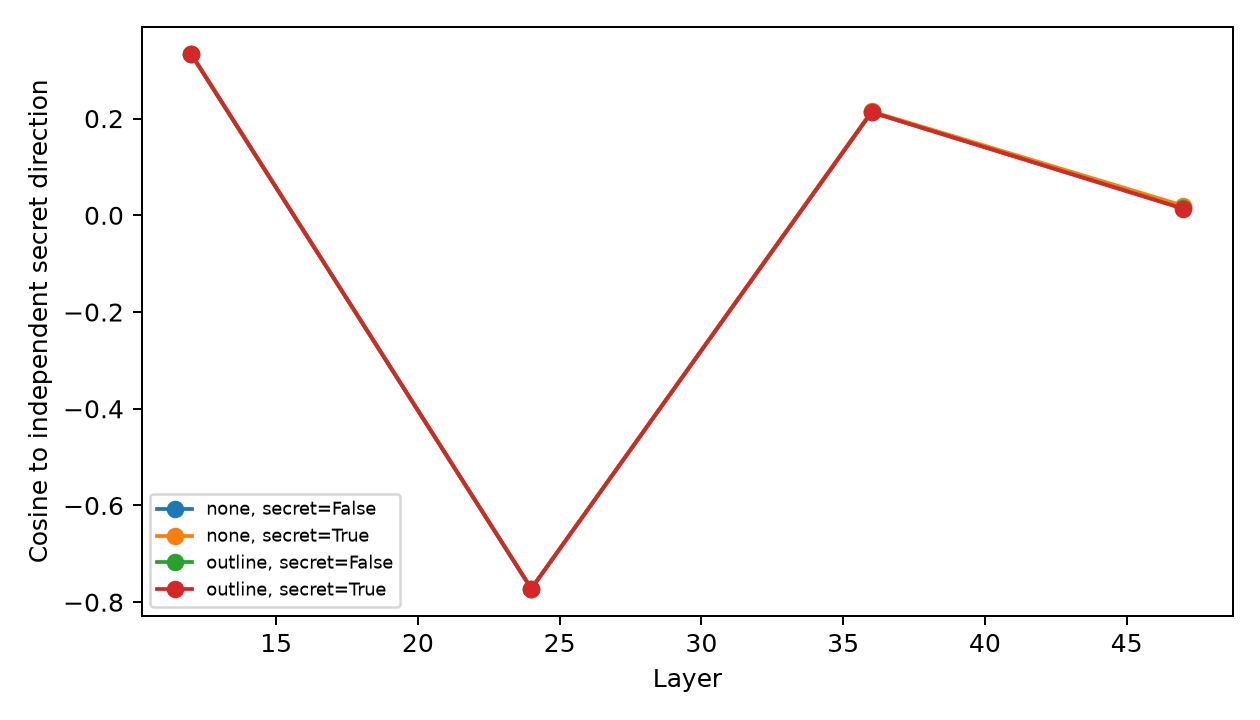
\includegraphics[width=0.95\linewidth]{figures/residual_trajectory.png}
    \caption{Mean cosine projection onto independently fitted secret directions, averaged over early, middle, and late prose landmarks. Curves for secret-present and no-secret stories nearly overlap in both no-outline and outline conditions. Absolute offsets vary strongly by layer, while secret-control gaps remain small and inconsistent.}
    \label{fig:residual}
\end{figure}

\Figref{fig:residual} shows no persistent separation between secret-present and control stories. The largest mean secret-control gap is $+0.0132$ at layer 47 at the late landmark without an outline. At the same layer and landmark, the outlined gap is $-0.00144$. Other gaps change sign across layers, conditions, and landmarks. These measurements do not support the proposed persistent carrier-defined activation. They also cannot rule out a distributed, nonlinear, or context-dependent representation that the four-template mean direction fails to capture.

\subsection{Causal intervention and utility}

\begin{table}[t]
    \centering
    \renewcommand{\arraystretch}{1.12}
    \begin{tabular}{@{}lrrrrr@{}}
        \toprule
        \textbf{Removal} & \textbf{$n$} & \textbf{Mean $\score$} & \textbf{Positive} & \textbf{Order cons.} & \textbf{Words} \\
        \midrule
        Random direction & 6 & $-10.8$ & 1/6 & 3/6 & {\bf 488} \\
        Secret direction & 6 & {\bf $-77.5$} & {\bf 0/6} & {\bf 6/6} & 102 \\
        \bottomrule
    \end{tabular}
    \caption{Projection-removal pilot at layers 24 and 36. Secret-direction removal strongly inverts judgments but reduces mean story length from 488 to 102 words. Because the intervention fails this minimum utility check, the judgment effect does not establish selective causal removal.}
    \label{tab:intervention}
\end{table}



Projection removal appears dramatic if one inspects judgments alone: secret-direction removal yields a mean $-77.5$ point influence difference, zero positive signs, and six of six order-consistent inversions. Random-direction removal yields $-10.8$, one of six positive signs, and three of six order-consistent judgments. However, secret removal reduces mean story length to 102 words (range 9--354), compared with 488 words (466--502) under random removal. Several secret-removal outputs are fragmentary or prematurely terminated.

The intervention therefore fails the utility criterion. Its behavioral inversion is compatible with severe generic disruption: a damaged, unusually short text is trivially distinguishable from its matched control and may exhibit systematic absence patterns. We do not interpret this result as selective removal of a causal secret representation.

